\documentclass[a4paper]{article}
\usepackage{INTERSPEECH2014,amssymb,amsmath,epsfig}
\setcounter{page}{1}
\sloppy     % better line breaks
\ninept
%SM below a registered trademark definition
\def\reg{{\rm\ooalign{\hfil
     \raise.07ex\hbox{\scriptsize R}\hfil\crcr\mathhexbox20D}}}

%% \newcommand{\reg}{\textsuperscript{\textcircled{\textsc r}}}
\title{Speakers identification in broadcast TV: facilities and barriers}

%%%%%%%%%%%%%%%%%%%%%%%%%%%%%%%%%%%%%%%%%%%%%%%%%%%%%%%%%%%%%%%%%%%%%%%%%%
%% If multiple authors, uncomment and edit the lines shown below.       %%
%% Note that each line must be emphasized {\em } by itself.             %%
%% (by Stephen Martucci, author of spconf.sty).                         %%
%%%%%%%%%%%%%%%%%%%%%%%%%%%%%%%%%%%%%%%%%%%%%%%%%%%%%%%%%%%%%%%%%%%%%%%%%%
%\makeatletter
%\def\name#1{\gdef\@name{#1\\}}
%\makeatother
%\name{{\em Firstname1 Lastname1, Firstname2 Lastname2, Firstname3 Lastname3,}\\
%      {\em Firstname4 Lastname4, Firstname5 Lastname5, Firstname6 Lastname6,
%      Firstname7 Lastname7}}
%%%%%%%%%%%%%%% End of required multiple authors changes %%%%%%%%%%%%%%%%%

\makeatletter
\def\name#1{\gdef\@name{#1\\}}
\makeatother \name{{\em Author Name$^1$, Co-author Name$^2$}}

\address{$^1$Author Affiliation \\
  $^2$Co-author Affiliation \\
{\small \tt author@university.edu, coauthor@company.com}}

%\twoauthors{Karen Sp\"{a}rck Jones.}{Department of Speech and Hearing \\
%  Brittania University, Ambridge, Voiceland \\
%  {\small \tt Karen@sh.brittania.edu} }
%  {Rose Tyler}{Department of Linguistics \\
%  University of Speechcity, Speechland \\
%  {\small \tt RTyler@ling.speech.edu} }

%
\begin{document}
\maketitle
%
\begin{abstract}
...
\end{abstract}
\noindent{\bf Index Terms}: speaker recognition, error analysis


\section{Introduction}

\section{\label{notation}Notation}

\begin{tabular}{|c|l|}
\hline 
Notation & Description \\ 
\hline 
\hline
$SpkShow$ & All speech segments of a speaker in a video \\ 
$SpkSeg$  & A speaker turn \\
$T^{ref}_i$ & the total duration of the speech\\
& of  $SpkShow_i$, in the reference \\
$T^{test}_i$ & the total duration where $SpkShow_i$\\
& is recognized by the automatic system\\
$T^{corr}_i$ & the total duration of correct\\
& identification of $SpkShow_i$\\

\hline 
\end{tabular} 

 
\section{Systems description}
brief description of the systems: training data, modelling, decision...
\subsection{PERCOL}

\subsection{QCOMPERE}

\subsection{SODA}


\section{Performance analysis}
we are interested here in analyzing the performances obtained per speaker, according to their characteristics, for instance in terms of speech turns etc. As the speech turns properties depend on the show in which the speaker appears, one speaker in one show is considered as the unit of analysis, the so-called $SpkShow$. One speaker appearing in 2 different videos is considered as 2 distinct $SpkShow$.

The test corpus contains about 10 hours of annotated contents, on 62 different videos, totalizing 477 non-anonymous different $SpkShow$.

In the analysis, we adopt the point of view of the references: for each $SpkShow_i$ in the reference is computed a performance measure of the biometric system, defined as the F-measure of the detection of $SpkShow_i$. More precisely, considering the definition given in \ref{notation}, Precision and Recall can be computed for each $SpkShow_i$:
\begin{itemize}
\item $Precision_i=\frac{T^{corr}_i}{T^{test}_i}$
\item $Recall_i=\frac{T^{corr}_i}{T^{ref}_i}$
\item $Fm_i=\frac{2*Precision_i*Recall_i}{Precision_i+Recall_i}$
\end{itemize} 

Thus, $Fm_i=0$ means that $SpkShow_i$ was never correctly identified, whereas $Fm_i=1$ means that $SpkShow_i$ is perfectly identified, without miss detection nor false alarm.

The table \ref{table-spkshow-perf} shows the average $Fm$ per $SpkShow$ for the different systems.
\begin{table*}[t]
\begin{center}
\begin{tabular}{r||c|c|c}
& Percol & Qcompere & Soda \\\hline\hline
average $Fm$ & 0.361 & 0.381 & 0.351\\\hline
average $Fm$ for in dictionary speakers & 0.628 & 0.684 & 0.619\\\hline
\#$SpkShow$ out of dictionary & 200 & 209 & 204 \\\hline
\#$SpkShow$ in dictionary & 277& 268 & 273\\\hline
\#$SpkShow$ in dictionary, with $Fm=0$ & 79 & 63 & 86\\\hline
\end{tabular}
\caption{Average system performances per $SpkShow$}
\label{table-spkshow-perf}
\end{center}
\end{table*}

From the table we can notice the important number of $SpkShow$ which are not in the dictionary of the system, about 40\% for each system. As they don't have any model, they obviously cannot be identified, leading to an average global $Fm$ rather poor. More interestingly, the number of $SpkShow$ which are actually in the dictionary and which are not recognised at all, is not negligeable: their represent between 23.5\% to 31.5\% of the in-dictionary $SpkShow$, according to the systems.


The flgure \ref{PQS} plot the distribution of all the $SpkShow$ in the system dictionaries, according their performance $Fm$, for the different systems. Foreach $Spkshow$, the average performance and the maximal performance obtained across systems are computed, and the corresponding distribution are also plotted. We can see from this figure that the average performance presented in table\ref{table-spkshow-perf} is not at all representative of the performances obtained foreach $SpkShow$: speakers are either not recognized or well recognized. 

\begin{figure}[!h]
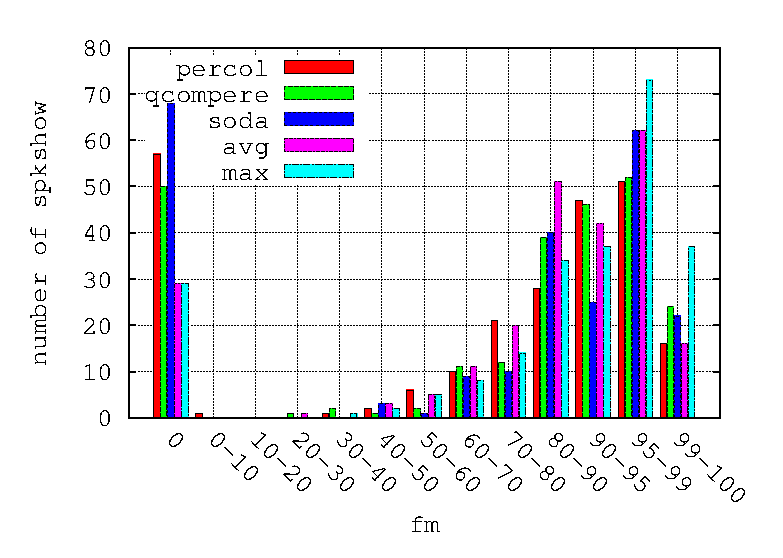
\includegraphics[scale=0.6]{PQS-mono-model.eps}
\caption{$spkShow$ performance distribution, for each system}
\label{PQS}
\end{figure}


\begin{figure}[!h]
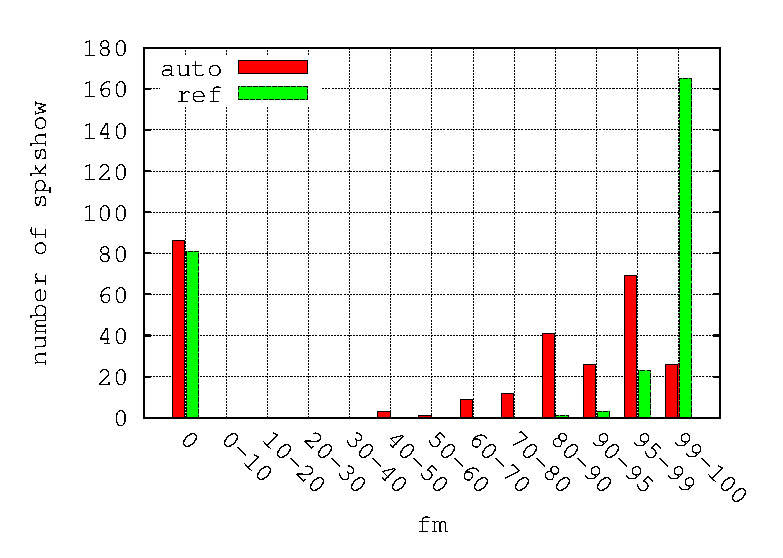
\includegraphics[scale=0.6]{SODA.eps}
\caption{$spkShow$ performance distribution, for SODA system, with reference and automatic speaker diarization}
\end{figure}

\begin{figure}[!h]
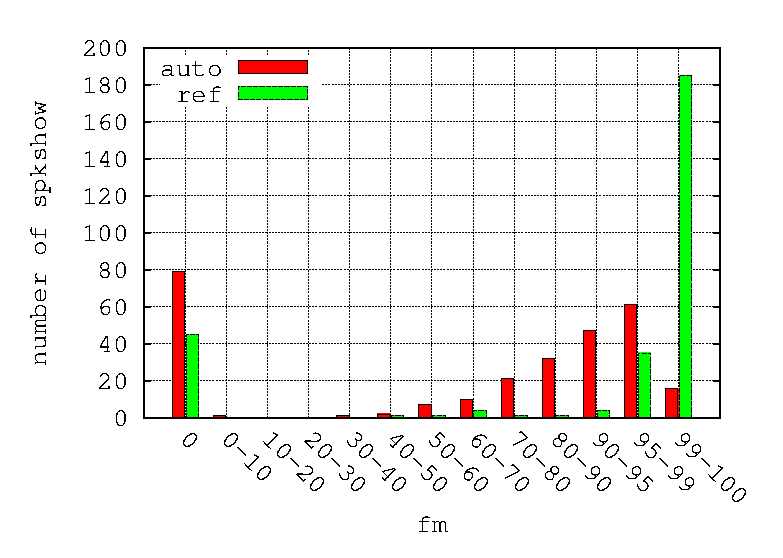
\includegraphics[scale=0.6]{PERCOL.eps}
\caption{$spkShow$ performance distribution, for PERCOL system, with reference and automatic speaker diarization}
\end{figure}




\section{Performance Prediction}

In this section, the aim is to predict the performance of the speaker, from his characteristics in terms of training data and speech turns properties. If we are able to predict, reliably, if the $Spkshow$ will be correctly recognized or not, when analysing on the main features contributing to this prediction, we can identify what are the features that  facilitates or hamper the identification, for a given system.

At each $SpkShow$ is associated the maximal $Fm$ obtained accross systems. Doing so, we do not focus on a particular system, but we try to explain "the-best-we-can-do" performance for each $SpkShow$.

\subsection{Detection}


\subsection{Prediction}

\section{Cross-show extension}





\section{Conclusions}



\section{Acknowledgements}


\newpage

\eightpt
\bibliographystyle{IEEEtran}

\begin{thebibliography}{10}

\bibitem[1]{ES1} ....

\end{thebibliography}
\end{document}
